\section{Introduction}
System-on-Chip (SoC) design lies at the heart of modern computing systems, enabling efficient integration of processors, accelerators, and interconnects onto a single chip for domain-specific applications. However, designing an SoC is an inherently complex and multidisciplinary task \cite{soc-productivity}, typically requiring close collaboration among experts in hardware architecture, embedded software, performance optimization, and integrated circuit design. As application demands for both performance and energy efficiency continue to grow while semiconductor technology scaling slows down \cite{esmaeilzadeh2011dark} \cite{hardavellas2012rise}, SoCs must integrate increasingly heterogeneous components to meet stringent performance, power, and area (PPA) requirements. This growing complexity introduces significant challenges across multiple stages of the SoC design flow \cite{soc-challenges}, necessitating more intensive cross-layer optimizations. 

To mitigate the challenges, several SoC design tools have been proposed \cite{esp4ml, chipyard, 10.1145/3400302.3415753}. ESP platform \cite{10.1145/3400302.3415753} provides a semi-automated SoC design and prototyping flow, enabling streamlined integration from hardware/software development to full-system validation on FPGAs. ESP4ML\cite{esp4ml} presents an open-source, fully-automated design flow that integrates ESP and HLS4ML \cite{fahim2021hls4mlopensourcecodesignworkflow} to enable SoC architectures for embedded machine learning applications. Chipyard \cite{chipyard} is another open-source, extensible framework for designing, simulating, and prototyping SoC architectures, built around the RISC-V ecosystem and Chisel hardware construction language \cite{Chisel}. Despite these advancements in automatic SoC integration and prototyping, the major SoC design challenges including design requirements interpretation, IP selection, hardware/software partitioning, customized accelerator generation, and the high-dimensional SoC design space exploration (DSE) still require extensive handcrafted design and demand multiple-discipline domain expertise and thorough understanding of tool-specific methodologies that limit accessibility and slow down the overall SoC development.

%这部分文献需要更新吗？

Recent breakthroughs in large language models (LLMs) \cite{minaee2025largelanguagemodelssurvey} offer a compelling new opportunity to rethink SoC design automation. LLMs have demonstrated strong capabilities in code generation, tool usage, and multistep reasoning, making them powerful agents for guiding technical workflows based on natural language instructions \cite{10.1145/3672459, 10.1145/3649476.3660393}. In the hardware domain \cite{Chen_2024}, LLMs have shown promise in HDL code generation \cite{blocklove2025automaticallyimprovingllmbasedverilog, 10.1145/3625223.3649280}, high-level synthesis \cite{xiong2024hlspilot, collini2024c2hlscleveraginglargelanguage}, design validation \cite{10473893, 10779517}, CPU design and verification \cite{processor-verification, ChatCPU}, AI accelerator generation \cite{10323953}, and RTL-level error diagnosis and repair \cite{tsai2024rtlfixerautomaticallyfixingrtl}.
%这个地方是不是改成把现在有一部分已经探索soc
While these works have primarily focused on small-scale RTL design components and processors with well-studied architectures, a fully automated SoC integration flow remains lacking due to the need for multidisciplinary knowledge and expertise. However, their ability to coordinate multistage development workflows \cite{computers14030094} suggests a similar potential for orchestrating SoC design processes.

Beyond their technical strengths, LLM-based automation has the potential to improve the economics of SoC development. Non-recurring engineering (NRE) costs include upfront expenditures on software development, IP licensing, chip design, verification, and mask production \cite{chen2025chipletsurvey}. High design and verification costs pose a substantial barrier to specialized hardware for smaller markets, motivating methods that lower development costs and shorten design cycles \cite{shalf2020future}. By automating labor-intensive design tasks, LLM agents could reduce the engineering-effort component of NRE and help make customized SoCs more economically accessible to lower-volume, domain-specific applications. This potential provides an additional motivation for SoCPilot, alongside its technical objectives of coordinating application analysis, hardware generation, and system-level optimization. Figure~\ref{fig:nre-break-even} illustrates this opportunity using the simplified unit-cost model $C(Q)=N/Q+c$, where $N$ is NRE, $Q$ is production volume, and $c$ is recurring cost per unit. Against an off-the-shelf alternative with unit cost $C_{\mathrm{alt}}>c$ and negligible incremental NRE, the break-even volume is $Q^*=N/(C_{\mathrm{alt}}-c)$. Reducing design-related NRE can therefore shift the break-even point toward smaller production volumes, assuming unchanged recurring unit costs and comparable application requirements.

\begin{figure}[t]
    \centering
    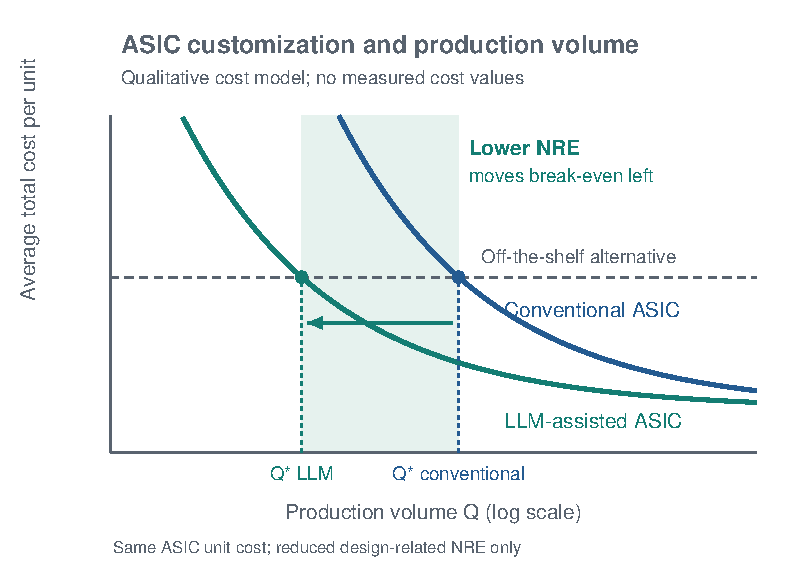
\includegraphics[width=\columnwidth]{pic/nre-break-even.pdf}
    \caption{Conceptual effect of LLM-assisted design on ASIC economics. Lower design-related NRE reduces amortized unit cost and shifts the break-even production volume to the left. The shaded interval indicates volumes where customization becomes cost-competitive only after NRE reduction. Curves are illustrative, not measured; recurring ASIC unit cost and the off-the-shelf alternative are held fixed.}
    \label{fig:nre-break-even}
\end{figure}


Motivated by both the technical and economic potentials, we propose SoCPilot, an LLM-powered framework for application-driven CPU--accelerator SoC customization and FPGA validation. SoCPilot begins by interpreting user requirements and selecting appropriate IPs through semantic search and library matching. It then performs hardware/software partitioning using application profiling, accelerator latency and area estimation, and communication-aware cost evaluation. For hardware-mapped tasks, the LLM generates ESP-compatible accelerators \cite{10.1145/3400302.3415753, esp4ml}, while system-level DSE refines processor, cache, and accelerator parameters under area constraints. The selected SoC is finally synthesized and validated on an FPGA board. By automating application analysis, hardware generation, architectural selection, and SoC integration, SoCPilot reduces the cross-layer engineering effort required to construct customized CPU--accelerator systems.

This work makes the following key contributions.
\begin{itemize}
\item We propose \textbf{SoCPilot}, an application-driven LLM-powered framework that automates application analysis, hardware/software partitioning, accelerator generation, and heterogeneous SoC configuration and integration.

\item SoCPilot combines runtime profiling, communication-aware partitioning, accelerator generation, and system-level design space exploration to select CPU--accelerator configurations under latency and area objectives.

\item Experimental results on representative applications demonstrate that SoCPilot-generated SoCs can be validated on an FPGA board and provide significant end-to-end performance improvements over matched CPU-only execution.
\end{itemize}



